\documentclass{article}
\usepackage[UTF8]{ctex}
\usepackage{tikz}
\usepackage{caption}
\usepackage{amsmath}
\usepackage{hyperref}
\usepackage{titlesec}
\usepackage{graphicx}
\usepackage[total={7in,10in}]{geometry}
\usepackage{subcaption}
\usepackage{mathtools}
\usepackage{amssymb}
\usepackage{xcolor}

\newcounter{para}
\newcommand\mypara{\par\refstepcounter{para}(\thepara)\space}
\titleformat{\section}[block]{\Large\bfseries\filcenter}{}{0em}{}
\renewcommand\thesection{}
\renewcommand\thesubsection{\protect\setcounter{equation}{0}\protect\setcounter{para}{0}第 \arabic{subsection} 题}

\usetikzlibrary{decorations.markings}

\tikzset{gradient/.style n args={2}{
    postaction={
        decorate,
        decoration={
            markings,
            mark=between positions 0 and \pgfdecoratedpathlength step 0.5pt with {
                \pgfmathsetmacro\myval{multiply(divide(
                    \pgfkeysvalueof{/pgf/decoration/mark info/distance from start}, \pgfdecoratedpathlength),100)};
                \pgfsetfillcolor{#2!\myval!#1};
                \pgfpathcircle{\pgfpointorigin}{1pt};
                \pgfusepath{fill};}
}}}}

\title{hs\_phys\_probs 002}
\author{詹有丘}
\date{}

\begin{document}

\maketitle

\subsection{太空跳绳}
一根不可伸长的长度为 $l$, 质量为 $m$ 的均质软绳, 两端固定在间隔为 $b$ 的两点.
绳子以两个固定点的连线为轴以匀角速度 $\omega$ 转动.
忽略重力的影响而只考虑离心力.
转动过程中绳子的形状保持为一个平面图形不变.
(本题可以以积分及隐函数形式给出隐式解.)

\mypara
用平面坐标系中的方程描述绳子的形状.

\mypara
求绳子的动能.

\mypara
求固定点处对绳子的拉力的大小.

\subsection{地铁站闸机}
某地铁站的出入站闸机采用三锟闸设计.
三锟闸是这样一种装置:
考虑三维空间中的三根长度均为 $l$ 的细硬轻杆, 每根杆都有一端被固定在点 $O$ 处,
且它们两两之间的夹角被固定为 $\alpha$.
显然存在一条过 $O$ 的轴 $z$ 使得三锟闸绕 $z$ 轴有 $\frac{2\pi}3$ 旋转对称.
$z$ 轴与地面的夹角被适当地选取, 以至于三锟闸在初始状态可以与地面达成这样一种相对位形:
其中一根杆与地面平行, 另外两根杆的自由端的连线也与地面平行.
有一堵固定在地面上的墙, 其位置满足:
在初始状态下, 三锟闸的水平杆垂直于墙, 且墙面紧贴在水平杆的自由端.
将通过闸机的人简化为刚性长方体.
人通过闸机的过程中, 长方体推动三锟闸绕 $z$ 轴转动, 长方体的一个面紧贴地面, 另一个面紧贴墙面.
长方体足够高.

\mypara
求满足以下条件的长方体的最大宽度 $a_0$: 人能完全通过闸机, 且长方体的厚度可以任意大.

\mypara
接上问, 若长方体的宽度 $a>a_0$, 求满足以下条件的长方体的最大横截面积: 人能完全通过闸机.

\mypara
若长方体的宽度为 $a$, 人在完全通过闸机的过程中需要克服三种摩擦:
来自墙面和地面的滑动摩擦力 (大小恒定为 $f$),
来自杆的滑动摩擦力 (摩擦系数为 $\mu$),
来自三锟闸转轴的滑动摩擦力矩 (大小恒定为 $K$).
求人在缓慢地完全通过闸机的过程中, 来自杆的滑动摩擦耗散的能量为多少.

\subsection{Hohmann 转移轨道}
质量为 $m$ 的物体一开始绕着质量为 $M\gg m$ 的星体在半径为 $r_1$ 的圆轨道上运动.
某时其瞬间加速, 使速度方向不变, 速率增大 $\Delta v_1$, 进入椭圆轨道.
在远心点处, 其再次瞬间加速, 使速度方向不变, 速率增大 $\Delta v_2$,
进入半径为 $r_2=xr_1$ 的圆轨道上运动.
证明使 $\Delta v_1+\Delta v_2$ 最大的 $x$ 为
$5+4\sqrt7\cos\!\left(\frac13\arctan\frac{\sqrt3}{37}\right)$.

\subsection{电容势函数}
有一平行板电容器.
定义变量 $X$ 为极板间距, $Q$ 为一个极板上的电荷量大小,
$F$ 为极板间作用力, $V$ 为极板间的电势差.
电容 $C\!\left(X\right)$ 是已知函数 (不一定是反比例函数).
定义势函数 $U$ 为电容器储存的能量.

\mypara
证明 $\mathrm dU=V\,\mathrm dQ-F\,\mathrm dX$.

\mypara
证明 $\left(\frac{\partial V}{\partial F}\right)_Q=\left(\frac{\partial X}{\partial Q}\right)_F$.

\mypara
若 $C\!\left(X\right)$ 是反比例函数,
在 $F$-$X$ 图中分别作出等 $V$ 过程和等 $Q$ 过程的图像.

\subsection{张拉整体}
张拉整体 (tensegrity) 是一个由一些互不触碰的受压结构 (刚体) 以及连接它们的受拉结构 (绳) 组成的稳定结构.
其在建筑学, 工程学, 生物学等领域都有应用.
图 \ref{fig:张拉整体} (Cmglee, 2012) 是一个例子,
其由顶部和底部各一个边长为 $a$ 的正 $n$ 边形 (图中 $n=4$) 组成.
记底面的正 $n$ 边形为多边形 $\mathrm A_0\cdots\mathrm A_{n-1}$,
顶面上的正 $n$ 边形为多边形 $\mathrm B_0\cdots\mathrm B_{n-1}$.
$\mathrm A_0$ 与 $\mathrm A_n$ 是同一个点,
$\mathrm B_0$ 与 $\mathrm B_n$ 是同一个点.
对每个 $j$, 用长度为 $b$ 的轻绳连接 $\mathrm A_j\mathrm B_j$,
用长度为 $l$ 的轻杆连接 $\mathrm A_j\mathrm B_{j+1}$.

\mypara
多边形 $\mathrm A_0\cdots\mathrm A_{n-1}$ 在旋转一定角度 (旋转的方向与 $\mathrm A_j$ 随 $j$ 变化的环绕方向相同) 之后,
可以平移至与多边形 $\mathrm B_0\cdots\mathrm B_{n-1}$ 重合.
求该转角的最小正值.

\mypara
记 $T\!\left(\mathrm{PQ}\right)$ 为连接 $\mathrm P,\mathrm Q$ 两点的绳或杆上的力,
正值表示张力, 负值表示压力.
已知, 对每个 $j$, $T\!\left(\mathrm A_j\mathrm A_{j+1}\right)=T_0$.
对每个 $j$, 求 $T\!\left(\mathrm A_j\mathrm B_j\right)$ 和 $T\!\left(\mathrm A_j\mathrm B_{j+1}\right)$.

\begin{figure}[h!]
	\centering
	\includegraphics[width=0.5\linewidth]{Tensegrity_simple_4_RL.png}
	\caption{}
	\label{fig:张拉整体}
\end{figure}

\subsection{彩色视觉}

视觉感受器 (眼睛) 中对彩色视觉至关重要的生物基础是视锥细胞 (corn cell).
在光线充足的情况下, 视锥细胞比视杆细胞 (rod cell) 更加活跃,
我们因此不考虑视杆细胞对视觉带来的影响.
某种动物的视网膜上有 $n$ 种视锥细胞, 从而可以产生 $n$ 色视觉 ($n$-chromacy)
(人类有三色视觉 (trichromacy),
梅花雀有四色视觉 (tetrachromacy)\footnote{
	Hart N. S., Partridge J. C., Bennett A. T., Cuthill I. C.\@.
	``Visual pigments, cone oil droplets and ocular media in four species of estrildid finch''.
	\textit{Journal of Comparative Physiology A}.
	Jul--Aug, 2000; \textbf{186} (7--8): 681--694.
	doi: 10.1007/s003590000121. PMID: 11016784. S2CID: 19458550.
},
青凤蝶 (\textit{Graphium sarpedon}) 有十五色视觉\footnote{
	Chen P., Awata H., Matsushita A., Yang E., Arikawa K.\@.
	``Extreme Spectral Richness in the Eye of the Common Bluebottle Butterfly, \textit{Graphium sarpedon}''.
	\textit{Frontiers in Ecology and Evolution}, vol. 4, pp. 18. Mar 8, 2016.
	doi: 10.3389/fevo.2016.00018. ISSN: 2296-701X.
}).
第 $j$ 种视锥细胞对波长为 $\lambda$ 的光的吸收率为 $f_j\!\left(\lambda\right)$,
其中 $f_j$ 看作 $\mathbf f:\left(0,+\infty\right)\to\left[0,1\right]^n$ 的第 $j$ 个分量.
$\left\{f_j\right\}$ 是线性无关的.

第 $j$ 种视锥细胞在某种光刺激下的响应程度正比于它从中吸收的总功率.
视锥细胞在受到刺激后, 会将响应信号以电信号的形式告诉大脑,
大脑即可获得视网膜上某处的各种视锥细胞的响应程度 $\mathbf c\in\left[0,+\infty\right)^n$,
其中 $\mathbf c$ 的分量 $c_j$ 为第 $j$ 种视锥细胞的响应程度.
从而颜色可以与 $C:=\left[0,+\infty\right)^n$ 中的向量一一对应.
特殊地, 我们称并不是每个分量都相同的 $\mathbf c$ 组成的集合为 $C^*$.

规定两种变换: $T_u:c_j\mapsto uc_j$ ($u>0$)
以及 $S_v:c_j\mapsto v\left(c_j-l\right)+l$ ($0<v\le\frac l{l-c_{\min}}$),
其中 $l$ 是 $\mathbf c$ 中最小分量 $c_{\min}$ 和最大分量 $c_{\max}$ 的平均值.
我们认为在这两种变换下 $\mathbf c$ 的色相保持不变.
我们在 $C^*$ 上关于色相建立一个等价关系: $\mathbf c\sim\mathbf c'$
当且仅当存在 $u,v$, 使得 $\mathbf c=T_uS_v\mathbf c'$.

设某种设备 (不妨称为彩灯) 能发出固定的 $n$ 种单色光, 其波长分别为 $\lambda_k$.
它能以任意不同的功率合成并发出这些单色光, 产生对视锥细胞的光刺激.

彩虹中包含了所有的单色光.

\mypara
设某个光刺激中能量随波长的分布为已知函数 $g\!\left(\lambda\right)$,
求该光刺激代表的颜色.

\mypara
求彩灯能产生的所有的颜色的集合 $L\subseteq C$.

\mypara
求彩虹中所有的颜色的集合 $R\subseteq C$.

\mypara
若存在一组 $\left\{\lambda_k\right\}$, 使得 $L=C$.
求 $\mathbf f$ 需要满足的条件.

\mypara
是否对于任意的 $\mathbf c\in C^*$, 存在 $\mathbf c'\in R$, 使得 $\mathbf c\sim\mathbf c'$?
若是, 给出构造 $\mathbf c'$ 的方法.
若否, 是否对于 $C^*$ 中的任意具有一块有限体积的区域 $D$,
对于几乎所有的 $\mathbf c\in D$, 不存在这样的 $\mathbf c'$?

\mypara
是否对于任意的 $\mathbf c\in C^*$, 存在 $\mathbf c'\in L$, 使得 $\mathbf c\sim\mathbf c'$?
若是, 给出构造 $\mathbf c'$ 的方法.
若否, 是否对于任意的 $\mathbf c\in R$, 存在 $\mathbf c'\in L$, 使得 $\mathbf c\sim\mathbf c'$?

\subsection{互 LC 震荡}

我们知道电感有自感和互感.
但是, 虽然我们有``互电容''的概念, 其并不能与互感很好地对应.
我们现在来构造一种与互感相对应的概念``互容'':
考虑四块的面积为 $S$ 的平行极板, 依次编号为 a--d.
极板 a 和极板 c 看作一个电容器, 极板间距为 $d_1$;
极板 b 和极板 d 看作一个电容器, 极板间距为 $d_2$;
极板 b 和极板 c 的间距为 $d$.

\mypara
求这两个电容器之间的互容系数.

\mypara
设有两个 LC 电路,
电路中分别有电容 $C_1$ 与 $C_2$, 电感 $L_1$ 与 $L_2$.
两个电容之间的互容系数为 $N$, 两个电感之间的互感系数为 $M$.
设在 $t=0$ 时两个电容分别带电 $Q_{10}$ 与 $Q_{20}$,
求任意时刻 $t$ 时两个电容所带的电荷量 $Q_1\!\left(t\right)$ 与 $Q_2\!\left(t\right)$.

\subsection{球套黑球}

本题中提到的黑体都是余弦辐射体.
将一个热容为 $C$ 的半径为 $r$ 的均匀的球形的黑体 A
放在一个半径为 $R$ 的均匀的薄球壳 B 内.
两个球心的距离为 $d<R-r$.
在 $t=0$ 时, A 的温度为 $T_0$.
A 内部的热传导很快.

\mypara
B 是热容为 $D$, 初始温度为 $S_0$ 的黑体.
求 $t$ 时刻 A 的温度 $T\!\left(t\right)$.
(可保留代数方程, 积分, 微分方程等, 若数学计算过于复杂.)

\mypara
B 的内壁是可以完全反射热辐射的镜面.
求 $t$ 时刻 A 的温度 $T\!\left(t\right)$.

\newpage
\section{参考答案}

\subsection{太空跳绳}

\mypara
因为绳子的形状是具有最小势能的形状, 所以本题即求解最优化问题
\begin{alignat}{2}
	\min_{y\in C^1\left[-b/2,b/2\right]}\quad&
	\int_{-b/2}^{b/2}-\frac12\cdot\frac ml\sqrt{1+y'^2}\,\mathrm dx\cdot\omega^2\cdot y^2\\
	\mathrm{s.t.}\quad & y\!\left(-b/2\right)=y\!\left(b/2\right)=0,\\
	& \int_{-b/2}^{b/2}\sqrt{1+y'^2}\,\mathrm dx=l.
	\label{eq:绳长约束}
\end{alignat}
在目标函数中带上 Lagrange 乘子, 可以略去约束条件式 \ref{eq:绳长约束}, 而目标变为
\begin{alignat}{2}
	\max_{y\in C^1\left[-b/2,b/2\right]}\quad&
	\int_{-b/2}^{b/2}y^2\sqrt{1+y'^2}\,\mathrm dx-\lambda\left(\int_{-b/2}^{b/2}\sqrt{1+y'^2}\,\mathrm dx-l\right)\\
	\mathrm{s.t.}\quad & y\!\left(-b/2\right)=y\!\left(b/2\right)=0.
\end{alignat}

定义 Lagrangian
\begin{equation}
	\mathcal L:=\left(y^2-\lambda\right)\sqrt{1+y'^2}.
\end{equation}
代入 Euler--Lagrange 方程后化简可得
\begin{equation}
	2y\left(1+y'^2\right)=\left(y^2-\lambda\right)y''.
\end{equation}
进行变换 $p:=y'$ 后可得
\begin{equation}
	2y\left(1+p^2\right)=\left(y^2-\lambda\right)p\frac{\mathrm dp}{\mathrm dy}.
\end{equation}
分离变量并积分可得
\begin{equation}
	\ln\!\left(1+p^2\right)=2\ln\frac{a^2-y^2}{a^2-y_0^2},
	\label{eq:变分法}
\end{equation}
其中 $y_0:=y\!\left(0\right)>0$, $a:=\sqrt\lambda>y_0$.
回代 $p=y'$, 再次分离变量并积分可得
\begin{equation}
	\int_{y_0}^y\frac{\mathrm dy}{\sqrt{\left(\frac{a^2-y^2}{a^2-y_0^2}\right)^2-1}}=\pm x.
	\label{eq:曲线方程}
\end{equation}
式 \ref{eq:曲线方程} 给出描述绳子形状的方程.

约束条件 $y\!\left(-b/2\right)=y\!\left(b/2\right)=0$ 给出
\begin{equation}
	b=2\int_0^{y_0}\frac{\mathrm dy}{\sqrt{\left(\frac{a^2-y^2}{a^2-y_0^2}\right)^2-1}}.
	\label{eq:b约束}
\end{equation}
绳子上的长度微元
\begin{equation}
	\mathrm ds=\sqrt{1+y'^2}\,\mathrm dx
	=\frac{a^2-y^2}{a^2-y_0^2}\frac{\mathrm dy}{\sqrt{\left(\frac{a^2-y^2}{a^2-y_0^2}\right)^2-1}}
	=\frac{\mathrm dy}{\sqrt{1-\left(\frac{a^2-y_0^2}{a^2-y^2}\right)^2}}.
\end{equation}
从而
\begin{equation}
	l=2\int_0^{y_0}\frac{\mathrm dy}{\sqrt{1-\left(\frac{a^2-y_0^2}{a^2-y^2}\right)^2}}.
	\label{eq:l约束}
\end{equation}
式 \ref{eq:b约束} 与式 \ref{eq:l约束} 隐式给出了式 \ref{eq:曲线方程} 中的参数 $a$ 和 $y_0$.

\mypara
\begin{equation}
	E_\mathrm k=\int_{x=-b/2}^{b/2}\frac12\cdot\frac ml\,\mathrm ds\cdot \omega^2y^2
	=\frac{m\omega^2}{l}\int_0^{y_0}\frac{y^2\,\mathrm dy}{\sqrt{1-\left(\frac{a^2-y_0^2}{a^2-y^2}\right)^2}}.
\end{equation}

\mypara
质心位置为
\begin{equation}
	y_\mathrm c=\frac1m\int_{x=-b/2}^{b/2}y\cdot\frac ml\,\mathrm ds
	=\frac2l\int_0^{y_0}\frac{y\,\mathrm dy}{\sqrt{1-\left(\frac{a^2-y_0^2}{a^2-y^2}\right)^2}}
	=\frac{y_0\sqrt{2a^2-y_0^2}}l.
\end{equation}
绳子受到的合力
\begin{equation}
	F=m\omega^2y_\mathrm c
	=\frac{m\omega^2y_0\sqrt{2a^2-y_0^2}}l.
\end{equation}

在 $x=\pm b/2$ 处曲线的切线斜率
\begin{equation}
	y'\!\left(\pm b/2\right)=\mp\tan\theta=\mp\sqrt{\left(\frac{a^2}{a^2-y_0^2}\right)^2-1},
\end{equation}
从而固定点处对绳子的拉力大小
\begin{equation}
	T_{\pm b/2}=\frac F{2\sin\theta}
	=\frac{m\omega^2y_0\sqrt{2a^2-y_0^2}}{2l\sqrt{1-\left(\frac{a^2-y_0^2}{a^2}\right)^2}}
	=\frac{m\omega^2a}{2l}.
\end{equation}

\textit{另}: 此题可用受力法解.

\begin{figure}[h!]
	\centering
	\begin{tikzpicture}
		\draw[thick,->] (-1,0) -- (5,0) node[anchor=north] {$x$};
		\draw[thick,->] (0,-1) -- (0,5) node[anchor=east] {$y$};
		\draw[domain=0:2,smooth,variable=\x] plot ({\x}, {4-\x*\x/2});
		\draw[thick,->] (0,4) node[anchor=north east] {$y_0$} -- (-0.7,4) node[anchor=east] {$T_0$};
		\draw[thick,->] (1,3.5) -- (1,4.9) node[anchor=west] {$\int_0^x\frac ml\,\mathrm ds\cdot\omega^2\cdot y$};
		\draw[dashed] (2,2) node[anchor=north west] {$\theta$} -- (3,2);
		\draw[thick,->] (2,2) -- (2.7,0.6) node[anchor=west] {$T$};
	\end{tikzpicture}
	\caption{}
	\label{fig:绳子受力分析}
\end{figure}

设绳子在 $x=0$ 处的张力为水平方向 $T_0$,
考虑 $\left[0,x\right]$ 上的一段绳子的受力平衡, 如图 \ref{fig:绳子受力分析} 所示.
考虑到 $\tan\theta=-y'$, 有
\begin{equation}
	\int_0^x\frac ml\,\mathrm ds\cdot\omega^2\cdot y=-T_0y'.
\end{equation}
两边对 $x$ 求导可得
\begin{equation}
	\frac{m\omega^2}{l}\sqrt{1+y'^2}=-T_0y''.
\end{equation}
变换 $p:=y'$, 分离变量得
\begin{equation}
	\frac{p\,\mathrm dp}{\sqrt{1+p^2}}=-\frac{m\omega^2}{T_0l}y\,\mathrm dy.
\end{equation}
两边积分得
\begin{equation}
	\sqrt{1+p^2}-1=-\frac{m\omega^2}{2T_0l}\left(y^2-y_0^2\right).
	\label{eq:受力法}
\end{equation}
代换 $a:=\sqrt{\frac{2T_0l}{m\omega^2}+y_0^2}$ 可将式 \ref{eq:受力法} 变为与式 \ref{eq:变分法} 等价的形式.

\subsection{地铁站闸机}

\subsection{Hohmann 转移轨道}

物体的速度变化的全过程为
\begin{equation}
	\underbrace{\sqrt{\frac{GM}{r_1}}}_{\text{圆轨道}}\xrightarrow{\Delta v_1}
	\underbrace{\sqrt{-\frac{2GM}{r_1+r_2}+\frac{2GM}{r_1}}
	\rightarrow\sqrt{-\frac{2GM}{r_1+r_2}+\frac{2GM}{r_2}}}_{\text{椭圆轨道}}
	\xrightarrow{\Delta v_2}\underbrace{\sqrt{\frac{GM}{r_2}}}_{\text{圆轨道}}.
\end{equation}

于是
\begin{equation}
	\Delta v_1+\Delta v_2\propto f\!\left(x\right):=
	\sqrt{\frac{2x}{1+x}}-1+\sqrt{\frac1x}-\sqrt{\frac2{x\left(1+x\right)}}.
\end{equation}
为了使 $\Delta v_1+\Delta v_2$ 极大,
\begin{equation}
	f'\!\left(x\right)=-\frac12x^{-\frac32}-\frac1{\sqrt2}x^{-\frac12}\left(1+x\right)^{-\frac32}
	+\frac1{\sqrt2}\left(1+2x\right)x^{-\frac32}\left(1+x\right)^{-\frac32}=0.
	\label{eq:f'(x)=0}
\end{equation}
在式 \ref{eq:f'(x)=0} 两边乘 $2x^{\frac32}\left(1+x\right)^{\frac32}$ 可得
\begin{equation}
	\sqrt2\left(1+3x\right)-\left(1+x\right)^{\frac32}=0.
\end{equation}
此方程可约化为多项式方程
\begin{equation}
	P\!\left(x\right):=x^3-15x^2-9x-1=0.
\end{equation}

注意到
\begin{equation*}
	\cos3y=\cos y\left(2\cos^2y-1\right)-2\cos y\left(1-\cos^2y\right)=4\cos^3y-3\cos y,
\end{equation*}
所以
\begin{equation*}
	\cos^3\frac y3=\frac14\left(\cos y+3\cos\frac y3\right).
\end{equation*}

令 $x^\star:=5+4\sqrt7\cos\!\left(\frac13\arctan\frac{\sqrt3}{37}\right)$, 则
\begin{align}
	\left(x^\star-5\right)^3&=16\cdot 7^{\frac 32}\left(\cos\arctan\frac{\sqrt3}{37}+3\cos\!\left(\frac13\arctan\frac{\sqrt3}{37}\right)\right)\\
	&=16\cdot 7^{\frac 32}\left(\frac{37}{2\cdot 7^{\frac32}}+3\cdot\frac{x^\star-5}{4\sqrt7}\right)\\
	&=84x^\star-124.
\end{align}
由此可得 $P\!\left(x^\star\right)=0$.

\subsection{电容势函数}

\mypara
$V\,\mathrm dQ$ 是电源对电容所做的功, $-F\,\mathrm dX$ 是外力对电容所做的功.

\mypara
令 $H:=U+FX$, 则
\begin{equation}
	\mathrm dH=V\,\mathrm dQ+X\,\mathrm dF.
\end{equation}
从而
\begin{equation}
	V=\left(\frac{\partial H}{\partial Q}\right)_F,
	\qquad X=\left(\frac{\partial H}{\partial F}\right)_Q.
\end{equation}
由于求偏导次序可交换,
$\frac{\partial^2H}{\partial Q\partial F}=\frac{\partial^2H}{\partial F\partial Q}$,
因此
\begin{equation}
	\left(\frac{\partial V}{\partial F}\right)_Q=\left(\frac{\partial X}{\partial Q}\right)_F.
\end{equation}

\mypara
设 $C\!\left(X\right)=\alpha/X$, 则由 $Q=CV$ 可得状态方程
\begin{equation}
	QX=\alpha V.
\end{equation}
内能表达式为
\begin{equation}
	U=\frac12QV=\frac{Q^2X}{2\alpha}.
\end{equation}
于是
\begin{equation}
	F=-\left(\frac{\partial U}{\partial X}\right)_Q=\frac{Q^2}{2\alpha}=\frac{\alpha V^2}{2X^2}.
\end{equation}
于是可以在 $F$-$X$ 图作出如图 \ref{fig:电容势函数的图} 所示的曲线.
图 \ref{fig:等V过程} 与图 \ref{fig:等Q过程} 分别是等 $V$ 过程与等 $Q$ 过程的图像.

\begin{figure}[h!]
	\centering
	\begin{subfigure}[b]{0.4\linewidth}
		\centering
		\begin{tikzpicture}
			\draw[thick,->] (0,0) -- (5,0) node[anchor=north] {$X$};
			\draw[thick,->] (0,0) -- (0,4) node[anchor=east] {$F$};
			\draw[domain=0.9:4.5,smooth,variable=\x] plot ({\x},{3/\x/\x});
		\end{tikzpicture}
		\caption{等 $V$ 过程}
		\label{fig:等V过程}
	\end{subfigure}
	\begin{subfigure}[b]{0.4\linewidth}
		\centering
		\begin{tikzpicture}
			\draw[thick,->] (0,0) -- (5,0) node[anchor=north] {$X$};
			\draw[thick,->] (0,0) -- (0,4) node[anchor=east] {$F$};
			\draw (0.5,2.5) -- (4.5,2.5);
		\end{tikzpicture}
		\caption{等 $Q$ 过程}
		\label{fig:等Q过程}
	\end{subfigure}
	\caption{}
	\label{fig:电容势函数的图}
\end{figure}

\subsection{张拉整体}

\subsection{彩色视觉}

\mypara
\begin{equation}
	\mathbf c=\int_0^\infty\mathbf f\!\left(\lambda\right)g\!\left(\lambda\right)\mathrm d\lambda.
\end{equation}

\mypara
\begin{equation}
	L=\left\{\sum_ka_k\mathbf f\!\left(\lambda_k\right)\,\middle|\,\mathbf a\in\left[0,+\infty\right)^n\right\}.
\end{equation}

\mypara
\begin{equation}
	R=\left\{a\mathbf f\!\left(\lambda\right)\,\middle|\,a\in\left[0,+\infty\right),\lambda\in\left(0,+\infty\right)\right\}.
\end{equation}

\mypara
$L=C$ 的充要条件是
\begin{equation}
	\forall j:\operatorname{supp}\!\left(f_j\right)\setminus
	\bigcup_{l\ne j}\operatorname{supp}\!\left(f_l\right)\ne\varnothing.
\end{equation}

充分性:
取
\begin{equation}
	\lambda_k:\in\operatorname{supp}\!\left(f_k\right)\setminus
	\bigcup_{l\ne k}\operatorname{supp}\!\left(f_l\right)
\end{equation}
即可.

必要性:
反证法.
若
\begin{equation}
	\operatorname{supp}\!\left(f_{j^*}\right)\setminus
	\bigcup_{l\ne j^*}\operatorname{supp}\!\left(f_l\right)=\varnothing,
\end{equation}
则显然对于 $c_j:=\delta_{j,j^*}$, 有 $C\ni\mathbf c\notin L$.

\mypara
首先考虑 $n=1$ 的情形.
此时显然有 $R=C$, 因此对于任意的 $\mathbf c\in C^*$,
存在与 $\mathbf c$ 等色相的 $\mathbf c'\in R$.

接下来考虑 $n=2$ 的情形.
此时显然有平凡的情形:
$\forall\mathbf c,\mathbf c'\in C^*:\mathbf c\sim\mathbf c'$.
又, $R$ 非空.
因此, 显然对于任意的 $\mathbf c\in C^*$,
存在与 $\mathbf c$ 等色相的 $\mathbf c'\in R$.

然后考虑 $n>3$ 的情形.
由于等价关系 $\mathbf c\sim\mathbf c'$ 中有两个可调参量 $u$, $v$,
所以对于任意的 $\mathbf c\in C^*$,
与 $\mathbf c$ 等色相的全体颜色组成的集合
\begin{equation}
	\left[\mathbf c\right]:=\left\{\mathbf c'\in C^*\,\middle|\,
	\mathbf c\sim\mathbf c'\right\}.
\end{equation}
是 $C$ 中的二维曲面.
又, 由于在 $R$ 上诱导的色相等价类 $\left[R\right]$
可以构造为 $C$ 中的一维曲线
(例如参数曲线 $\mathbf c=\mathbf f\!\left(\lambda\right)$
(参数 $\lambda\in\left(0,+\infty\right)$)).
当 $\mathbf c$ 在曲线 $\left[R\right]$ 上运动时,
二维曲面 $\left[\mathbf c\right]$ 将扫过一片三维超曲面 $P$.
显然 $P$ 可被定义为
\begin{equation}
	P:=\left\{\mathbf c\in C^*\,\middle|\,
	\exists\mathbf c'\in R:\mathbf c\sim\mathbf c'\right\}.
\end{equation}
由于 $P$ 是三维超曲面, 然而 $C$ 是 $n>3$ 维空间,
所以显然对于几乎所有的 $\mathbf c\in C^*$,
不存在与 $\mathbf c$ 等色相的 $\mathbf c'\in R$.

最后考虑 $n=3$ 的情形:

$n=3$ 是一个特殊的情形, 在这种情形中可以容易地构造一个函数
$p:C^*\to\left[-\pi,\pi\right)$
使得对于任意的 $\mathbf c,\mathbf c'\in C^*$,
有 $\mathbf c\sim\mathbf c'$ 当且仅当
$p\!\left(\mathbf c\right)=p\!\left(\mathbf c'\right)$.
构造方法如下:

定义
\begin{equation}
	\mathbf s\!\left(\mathbf c\right):=
	S_\frac{c_{\max}+c_{\min}}{c_{\max}-c_{\min}}\mathbf c,
	\quad\mathbf t\!\left(\mathbf c\right):=
	T_\frac1{c_{\max}}\mathbf c,
	\quad\mathbf u\!\left(\mathbf c\right):=\mathbf t\!\left(\mathbf s\!\left(\mathbf c\right)\right).
	\label{eq:标准化}
\end{equation}
此时 $\mathbf u$ 的作用是将 $\mathbf c\in C^*$ 标准化为满足
$c_{\min}=0$, $c_{\max}=1$ 的等色相的标准颜色
$\mathbf u\!\left(\mathbf c\right)$.
于是, 我们只需要为每一个标准颜色 $\mathbf c^\circ$
分配一个特征值 $q\!\left(\mathbf c^\circ\right)$, 即可定义出 $p$.
记 $\mathbf c$ 的三个分量为 $c_1,c_2,c_3$.
记对应于 $\mathbf c$ 的最小分量的下标为 $\min$,
对应于 $\mathbf c$ 的最大分量的下标为 $\max$.
定义 $q$ 为
\begin{equation}
	q\!\left(\mathbf c^\circ\right):=\frac\pi3\left(b+\varepsilon c^\circ_\mathrm{mid}\right),
\end{equation}
其中 $c_\mathrm{mid}$ 表示 $\mathbf c$ 中除了最大和最小以外的那个分量,
$b$ 与 $\varepsilon$ 的取值如表 \ref{tab:be} 所示.
从而, 可定义
\begin{equation}
	p\!\left(\mathbf c\right):=
	q\!\left(\mathbf u\!\left(\mathbf c\right)\right).
\end{equation}

\begin{table}[h!]
	\centering
	\begin{tabular}{c|ccc}
		$\min,\max$&$1$&$2$&$3$\\
		\hline
		$1$&&$2,1$&$-2,-1$\\
		$2$&$0,-1$&&$-2,1$\\
		$3$&$0,1$&$2,-1$&
	\end{tabular}
	\caption{}
	\label{tab:be}
\end{table}

此时各种情况都有可能出现.
可以对各种情况进行构造:
\begin{enumerate}
	\item
	按图 \ref{fig:吸收率a} 定义 $\mathbf f$,
	可知 $p\!\left(a\mathbf f\!\left(\lambda\right)\right)$
	可取遍 $\left[-\pi,\pi\right)$ 中的所有值,
	从而可以取遍所有的色相,
	从而对于所有的 $\mathbf c\in C^*$,
	存在与 $\mathbf c$ 等色相的 $\mathbf c'\in R$.

	\item
	按图 \ref{fig:吸收率b} 定义 $\mathbf f$,
	从而 $p\!\left(a\mathbf f\!\left(\lambda\right)\right)$
	只能取 $\left\{-\frac{2\pi}3,0,\frac{2\pi}3\right\}$ 中的值,
	从而对于几乎所有的 $\mathbf c\in C^*$,
	不存在与 $\mathbf c$ 等色相的 $\mathbf c'\in R$.

	\item
	将图 \ref{fig:吸收率a} 与图 \ref{fig:吸收率b} 各自取一半拼起来,
	从而并不是 $\forall\mathbf c\in C^*:\exists\mathbf c'\in R:\mathbf c\sim\mathbf c'$,
	但是, 也并不是对于所有的 $C^*$ 中具有一块有限体积的区域 $D$,
	对于几乎所有的 $\mathbf c\in D$,
	不存在与 $\mathbf c$ 等色相的 $\mathbf c'\in R$.
\end{enumerate}

\begin{figure}[h!]
	\centering
	\begin{subfigure}[b]{0.4\linewidth}
		\centering
		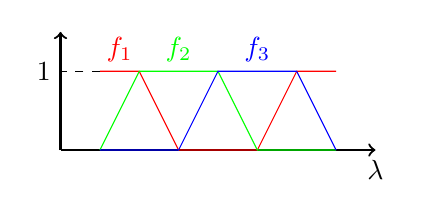
\begin{tikzpicture}
			\draw[thick,->] (0,0) -- (4,0) node[anchor=north] {$\lambda$};
			\draw[thick,->] (0,0) -- (0,1.5);
			\draw[red] (0.5,1) -- (1,1) -- (1.5,0) -- (2.5,0) -- (3,1) -- (3.5,1);
			\draw[green] (0.5,0) -- (1,1) -- (2,1) -- (2.5,0) -- (3.5,0);
			\draw[blue] (0.5,0) -- (1.5,0) -- (2,1) -- (3,1) -- (3.5,0);
			\draw[dashed] (0.5,1) -- (0,1) node[anchor=east] {$1$};
			\node[anchor=south] at (0.75,1) {$\color{red}f_1$};
			\node[anchor=south] at (1.5,1) {$\color{green}f_2$};
			\node[anchor=south] at (2.5,1) {$\color{blue}f_3$};
		\end{tikzpicture}
		\caption{}
		\label{fig:吸收率a}
	\end{subfigure}
	\begin{subfigure}[b]{0.4\linewidth}
		\centering
		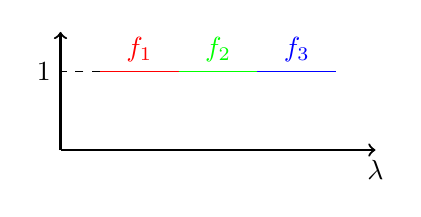
\begin{tikzpicture}
			\draw[thick,->] (0,0) -- (4,0) node[anchor=north] {$\lambda$};
			\draw[thick,->] (0,0) -- (0,1.5);
			\draw[red] (0.5,1) -- (1.5,1);
			\draw[green] (1.5,1) -- (2.5,1);
			\draw[blue] (2.5,1) -- (3.5,1);
			\draw[dashed] (0.5,1) -- (0,1) node[anchor=east] {$1$};
			\node[anchor=south] at (1,1) {$\color{red}f_1$};
			\node[anchor=south] at (2,1) {$\color{green}f_2$};
			\node[anchor=south] at (3,1) {$\color{blue}f_3$};
		\end{tikzpicture}
		\caption{}
		\label{fig:吸收率b}
	\end{subfigure}
	\caption{}
\end{figure}

\mypara
此题可以考虑 $C$ 中的几何直观.
首先应用式 \ref{eq:标准化} 给出的标准化方法,
映射 $\mathbf u$ 的像给出了一种用 $C$ 中的 $n-2$ 维超曲面表示
$C$ 上诱导的等价类 $\left[C\right]$ 的方法.
显然, $\mathbf u$ 的像由 $n\left(n-1\right)$ 个 $n-2$ 维超立方体组成:
\begin{equation}
	\operatorname{Im}\mathbf u=\bigcup_{j\ne l}\left\{\mathbf c\in C
	\,\middle|\,c_j=0,c_l=1,c_m\in\left[0,1\right],m\ne j,l\right\}.
\end{equation}
注意到变换 $S_v$ 可以将 $\operatorname{Im}\mathbf u$ 上的点 $\mathrm U$
变换到射线 $\mathrm PU$ 上的另外一点, 其中 $\mathrm P$ 是单位立方体的中心.
又, 变换 $T_u$ 可以将 $C$ 中的点 $\mathrm V$ 变换到射线 $\mathrm{OV}$ 上的另外一点.
从而, 与 $\mathbf c$ 等色相的颜色的集合 $\left[\mathbf c\right]$ 可以表为
$\angle\mathbf u\!\left(\mathbf c\right)\mathrm{OP}$ 所夹的二维平面区域
(不包括射线 $\mathrm{OP}$).
当 $\mathbf c$ 取遍所有的色相时, $\left[\mathbf c\right]$ 将扫过整个 $C^*$.

对于 $n=3$, 上面所述的几何直观由图 \ref{fig:三维色彩空间} 给出.
$\operatorname{Im}\mathbf u$ 即折线 $\mathrm{RYGCBMR}$.
当 $p\!\left(\mathbf c\right)$ 取遍 $\left[-\pi,\pi\right)$ 时,
$\mathbf u\!\left(\mathbf c\right)$ 沿着该折线绕 $\mathrm{OP}$ 转一圈.

\begin{figure}[h!]
	\centering
	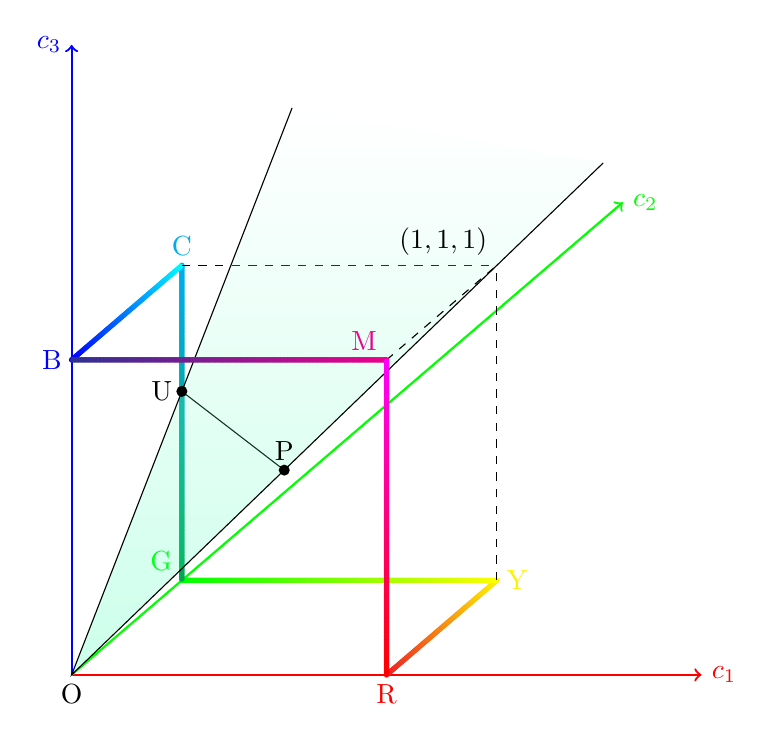
\begin{tikzpicture}[scale=2]
		\node[anchor=north] at (0,0) {O};
		\draw[red,thick,->] (0,0) -- (4,0) node[anchor=west] {$c_1$};
		\draw[green,thick,->] (0,0) -- (3.5,3) node[anchor=west] {$c_2$};
		\draw[blue,thick,->] (0,0) -- (0,4) node[anchor=east] {$c_3$};
		\path[gradient={red}{yellow}] (2,0) node[anchor=north] {\color{red}R} -- (2.7,0.6);
		\path[gradient={yellow}{green}] (2.7,0.6) node[anchor=west] {\color{yellow}Y} -- (0.7,0.6);
		\path[gradient={green}{cyan}] (0.7,0.6) node[anchor=south east] {\color{green}G} -- (0.7,2.6);
		\path[gradient={cyan}{blue}] (0.7,2.6) node[anchor=south] {\color{cyan}C} -- (0,2);
		\draw[dashed] (0.7,2.6) -- (2.7,2.6);
		\draw (1.35,1.3) -- (0.7,1.8);
		\draw[bottom color={rgb,1:red,0;green,1;blue,0.6},top color=white,fill opacity=0.2] (3.375,3.25) -- (0,0) -- (1.4,3.6);
		\draw[dashed] (2,2) -- (2.7,2.6);
		\path[gradient={blue}{magenta}] (0,2) node[anchor=east] {\color{blue}B} -- (2,2);
		\path[gradient={magenta}{red}] (2,2) node[anchor=south east] {\color{magenta}M} -- (2,0);
		\draw[dashed] (2.7,0.6) -- (2.7,2.6) node[anchor=south east] {$\left(1,1,1\right)$};
		\fill (1.35,1.3) node[anchor=south] {P} circle (1pt);
		\fill (0.7,1.8) node[anchor=east] {U} circle (1pt);
	\end{tikzpicture}
	\caption{}
	\label{fig:三维色彩空间}
\end{figure}

考虑到 $L$ 实际上是 $\left\{\mathbf f\!\left(\lambda_k\right)\right\}$
的 (具有非负系数的) 线性组合的集合.
因此, $L$ 是以 $\left\{\mathbf f\!\left(\lambda_k\right)\right\}$
各自延成的射线为棱边, 以 $\mathrm O$ 为顶点的超棱锥.
由几何直观可知, 当该超棱锥包含射线 $\mathrm{OP}$ 时
(即方程组 $\forall j:a_kf_j\!\left(\lambda_k\right)=1$
的解 $\mathbf a$ 的每个分量都是正的),
超棱锥内的点可以取遍所有的色相.
反之, 则不能.
因此, 对于任意的 $\mathbf c\in C^*$, 存在与 $\mathbf c$ 等色相的 $\mathbf c'\in L$
的条件是关于 $\mathbf a$ 的方程组 $\forall j:a_kf_j\!\left(\lambda_k\right)=1$
具有正的解.

不过这里我们认为 $\left\{\lambda_k\right\}$ 已经被选定而不能改变.
如果 $\left\{\lambda_k\right\}$ 可以被任意选定,
那么存在某种 $\mathbf f$ 的形式, 使得对于任意 $\left\{\lambda_k\right\}$ 的选择,
都并非对于任意的 $\mathbf c\in C^*$,
存在与 $\mathbf c$ 等色相的 $\mathbf c'\in L$.
例如, 我们可以构造一种 $\mathbf f$, 使得
$\forall\lambda:f_1\!\left(\lambda\right)>f_2\!\left(\lambda\right)$.
那么方程组 $\forall j:a_kf_j\!\left(\lambda_k\right)=1$
对任意的 $\left\{\lambda_k\right\}$ 都没有正的解.

若 $\left\{\lambda_k\right\}$ 的选取使得射线 $\mathrm{OP}$ 不被包含在超棱锥 $L$ 内,
则曲线 $\mathbf c=\mathbf f\!\left(\lambda\right)$ ($\lambda$ 为参数)
中的某一段可以处在超棱锥所能表达的色相之外.
该曲线也有可能完全处在超棱锥所表达的色相之内, 取决于 $\mathbf f$ 的具体形式.
因此, 若并不是对于任意的 $\mathbf c\in C^*$,
存在与 $\mathbf c$ 等色相的 $\mathbf c'\in L$,
那么对于可能对于任意的 $\mathbf c\in R$,
存在与 $\mathbf c$ 等色相的 $\mathbf c'\in L$,
这取决于 $\mathbf f$ 的形式.

\subsection{互 LC 震荡}

\subsection{球套黑球}

(此解答中球坐标的方位角取值为 $\left[-\pi,\pi\right)$.)

\mypara
如图 \ref{fig:黑体辐射} 所示, 以两个球心的连线为 $z$ 轴,
记 $\mathrm P$ 为 B 上 $x\mathrm Oz$ 平面内具有极角 $\theta$ 的点.
考虑 B 上 $\mathrm P$ 处单位面积发出的热辐射.

以 $\mathrm P$ 为原点建立坐标系, $z'$ 轴指向 $\mathrm O$.
平面 $x'\mathrm Pz'$ 与平面 $x\mathrm Oz$ 重合.
容易获得从 $x'y'z'$ 坐标系变换到 $xyz$ 坐标系的公式
\begin{equation}
	\left[\begin{matrix}x'\\y'\\z'\end{matrix}\right]=
	\left[\begin{matrix}-\cos\theta&0&-\sin\theta\\0&1&0
	\\\sin\theta&0&-\cos\theta\end{matrix}\right]
	\left(\left[\begin{matrix}x\\y\\z\end{matrix}\right]-
	R\left[\begin{matrix}\sin\theta\\0\\\cos\theta\end{matrix}\right]\right).
\end{equation}
于是 A 的球心 $\mathrm O_\mathrm A\left(x=d,y=0,z=0\right)$
在 $x'y'z'$ 坐标系中的坐标为
\begin{equation}
	\left[\begin{matrix}x'\\y'\\z'\end{matrix}\right]=
	\left[\begin{matrix}
		-\left(d-R\sin\theta\right)\cos\theta+R\cos\theta\sin\theta
		\\0\\\left(d-R\sin\theta\right)\sin\theta+R\cos^2\theta
	\end{matrix}\right]=
	\left[\begin{matrix}
		-d\cos\theta+R\sin2\theta
		\\0\\d\sin\theta+R\cos2\theta
	\end{matrix}\right].
\end{equation}

考虑从 $\mathrm P$ 发出的具有极角 $\theta'$ 和方位角 $\varphi'$ 的辐射.
该射线的参数方程为
\begin{equation}
	x'=s\sin\theta'\cos\varphi',\quad
	y'=s\sin\theta'\sin\varphi',\quad
	z'=s\cos\theta'.
\end{equation}
为了求该射线到 $\mathrm O_\mathrm A$ 的距离, 考虑该射线上的点 $\mathrm Q$,
其到 $\mathrm O_\mathrm A$ 的距离为
\begin{equation}\begin{split}
	\left|\mathrm{QO_A}\right|^2=
	&\left(-d\cos\theta+R\sin2\theta-s\sin\theta'\cos\varphi'\right)^2\\
	&+\left(-s\sin\theta'\sin\varphi'\right)^2\\
	&+\left(d\sin\theta+R\cos2\theta-s\cos\theta'\right)^2\\
	\ge&u\!\left(\theta,\theta',\varphi'\right).
\end{split}\end{equation}

其中 $u\!\left(\theta,\theta',\varphi'\right)$ 为 $\left|\mathrm{QO_A}\right|^2$
在 $s$ 变化时的最小取值 (二次函数最低点).
由方程 $u\!\left(\theta,\theta',\varphi'\right)=r^2$ 可以解得
$\theta'\in\left[0,\frac\pi2\right)$ 范围内的解
$\theta'=f\!\left(\theta,\varphi'\right)$.

$f$ 的形式在定性上有不同.
主要分为两种情形:

\begin{enumerate}

	\item
	$d<r$ 的情形:

	此时对于任意的 $\theta$, $z'$ 轴都会穿过 A.
	因此, $f$ 能定义在整个 $\left[0,\pi\right]\times\left[-\pi,\pi\right)$, 且是单值函数.

	\item
	$d\ge r$ 的情形:

	此时对于 $\theta\in\left[0,\arcsin\frac rd\right)\cup\left(\pi-\arcsin\frac rd,\pi\right]$,
	$z'$ 轴会穿过 A. 因此,
	$f$ 在 $\theta\in\left[0,\arcsin\frac rd\right)\cup\left(\pi-\arcsin\frac rd,\pi\right]$
	上是关于 $\varphi'\in\left[0,2\pi\right)$ 的单值函数.

	对于 $\theta\in\left[\arcsin\frac rd,\pi-\arcsin\frac rd\right]$, $z'$ 轴不穿过 A.
	因此, $f$ 在 $\theta\in\left[\arcsin\frac rd,\pi-\arcsin\frac rd\right]$ 上是关于
	$\varphi'\in\left[-\varphi'_\mathrm m\!\left(\theta\right),\varphi'_\mathrm m\!\left(\theta\right)\right]$
	的多值函数, 其有两支 $f_1$ 与 $f_2$.
	$f_1\le f_2$, 等号仅在 $\varphi'=\pm\varphi'_\mathrm m\!\left(\theta\right)$ 时取到.

\end{enumerate}

\begin{figure}[h!]
	\centering
	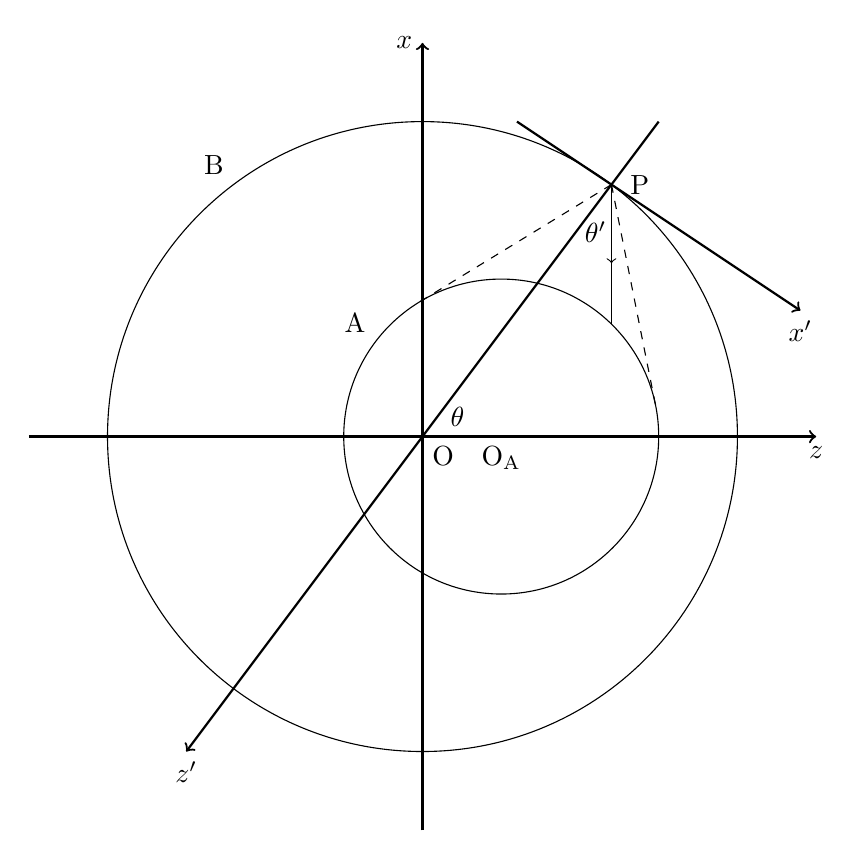
\begin{tikzpicture}
		\draw[thick,->] (-5,0) -- (5,0) node[anchor=north] {$z$};
		\draw[thick,->] (0,-5) -- (0,5) node[anchor=east] {$x$};
		\draw (0,0) circle (4);
		\node[anchor=south east] at (-0.6,1.2) {A};
		\draw (1,0) node[anchor=north] {$\mathrm O_\mathrm A$} circle (2);
		\node[anchor=south east] at (-2.4,3.2) {B};
		\node[anchor=south west] at (0,0) {~~$\theta$};
		\node[anchor=north west] at (0,0) {$\mathrm O$};
		\node[anchor=west] at (2.4,3.2) {~$\mathrm P$};
		\draw[thick,->] (3,4) -- (-3,-4) node[anchor=north] {$z'$};
		\draw[thick,->] (1.2,4) -- (4.8,1.6) node[anchor=north] {$x'$};
		\draw[dashed] (2.4,3.2) -- (-0.043,1.706);
		\draw[dashed] (2.4,3.2) -- (2.961,0.392);
		\draw[->] (2.4,3.2) -- (2.4,2.2);
		\node at (2.2,2.6) {$\theta'$};
		\draw (2.4,2.2) -- (2.4,1.428);
	\end{tikzpicture}
	\caption{}
	\label{fig:黑体辐射}
\end{figure}

B 在 $\mathrm P$ 处小面积 $\mathrm dA$ 的辐射中, 能射到 A 的功率为
\begin{equation}
	\mathrm dP_\mathrm{BA}\!\left(\theta\right)=
	L_\mathrm B\,\mathrm dA\cdot g\!\left(\theta\right),
\end{equation}
其中 $L_\mathrm B:=\frac\sigma\pi S^4$ 是温度为 $S$ 的黑体表面的辐射率 (单位面积上单位立体角的辐射通量),
$\mathrm dA:=R^2\sin\theta\,\mathrm d\theta\,\mathrm d\varphi$,
而
\begin{equation}
	g\!\left(\theta\right):=\begin{cases}
		\int_{\varphi'=-\pi}^{\pi}
		\int_{\theta'=0}^{f\!\left(\theta,\varphi'\right)}
		\cos\theta'\mathrm d\Omega,
		&\text{若 $d<r$, 或 $d\ge r$ 且
		$\theta\in\left[0,\arcsin\frac rd\right)\cup\left(\pi-\arcsin\frac rd,\pi\right]$;}\\
		\int_{\varphi'=-\varphi_\mathrm m'\!\left(\theta\right)}^{\varphi_\mathrm m'\!\left(\theta\right)}
		\int_{\theta'=f_1\!\left(\theta,\varphi'\right)}^{f_2\!\left(\theta,\varphi'\right)}
		\cos\theta'\mathrm d\Omega,
		&\text{若 $d\ge r$ 且 $\theta\in\left[\arcsin\frac rd,\pi-\arcsin\frac rd\right]$,}
	\end{cases}
\end{equation}
其中 $\mathrm d\Omega:=\sin\theta'\mathrm d\theta'\mathrm d\varphi'$.
从而 B 对 A 的总辐射功率为
\begin{equation}
	P_\mathrm{BA}=\int_{\theta=0}^\pi\int_{\varphi=-\pi}^{\pi}\mathrm dP_\mathrm{BA}\!\left(\theta\right),
\end{equation}
或者
\begin{equation}
	P_\mathrm{BA}=\lambda S^4,
\end{equation}
其中常数
\begin{equation}
	\lambda:=\begin{cases}
		\sigma R^2\int_0^\pi\sin\theta\,\mathrm d\theta
		\int_{-\pi}^\pi\mathrm d\varphi'
		\int_0^{f\!\left(\theta,\varphi'\right)}\sin\!\left(2\theta'\right)\mathrm d\theta',
		&\text{若 $d<r$;}\\
		\sigma R^2\left(
		\begin{matrix}\left(\int_0^{\arcsin\frac rd}+\int_{\pi-\arcsin\frac rd}^\pi\right)\sin\theta\,\mathrm d\theta
		\int_{-\pi}^\pi\mathrm d\varphi'
		\int_0^{f\!\left(\theta,\varphi'\right)}\sin\!\left(2\theta'\right)\mathrm d\theta'
		\\+\int_{\arcsin\frac rd}^{\pi-\arcsin\frac rd}\sin\theta\,\mathrm d\theta
		\int_{-\varphi'_\mathrm m\!\left(\theta\right)}^{\varphi'_\mathrm m\!\left(\theta\right)}\mathrm d\varphi'
		\int_{f_1\!\left(\theta,\varphi'\right)}^{f_2\!\left(\theta,\varphi'\right)}
		\sin\!\left(2\theta'\right)\mathrm d\theta'
		\end{matrix}\right),
		&\text{若 $d\ge r$.}
	\end{cases}
	\label{eq:黑体辐射参数}
\end{equation}

A 对 B 的总辐射功率显然为
\begin{equation}
	P_\mathrm{AB}=4\pi\sigma T^4r^2.
\end{equation}

B 对外耗散的总辐射功率显然为
\begin{equation}
	P_\mathrm{B\infty}=4\pi\sigma S^4R^2.
\end{equation}

从而可以建立微分方程组
\begin{equation}
	\begin{dcases}
		C\frac{\mathrm dT}{\mathrm dt}=P_\mathrm{BA}-P_\mathrm{AB},\\
		D\frac{\mathrm dS}{\mathrm dt}=P_\mathrm{AB}-P_\mathrm{BA}-P_\mathrm{B\infty},
	\end{dcases}
\end{equation}
即
\begin{equation}
	\begin{dcases}
		C\frac{\mathrm dT}{\mathrm dt}=\lambda S^4-4\pi\sigma T^4r^2,\\
		D\frac{\mathrm dS}{\mathrm dt}=4\pi\sigma T^4r^2-\lambda S^4-4\pi\sigma S^4R^2,
	\end{dcases}
	\label{eq:黑体辐射微分方程}
\end{equation}
其中 $\lambda$ 由式 \ref{eq:黑体辐射参数} 给出.
理论上可由式 \ref{eq:黑体辐射微分方程} 解出 $T\!\left(t\right)$.

\mypara
此情形给出平凡的结果
\begin{equation}
	T\!\left(t\right)=T_0.
\end{equation}
这是因为, A 的几乎全部辐射最终总能被反射回 A.
某根辐射在球形镜面内来回反射时, 它总在某个包含球心的平面内.
每一次反射的偏转角与 $2\pi$ 的比值我们可以假定为无理数 (因为几乎所有的实数都是无理数).
从而, 被反射的某根辐射可以稠密地铺满两个同心圆之间的区域.
该区域总是能与 A 有非空的交集 (因为一开始该辐射就是从 A 上射出的),
因此辐射总能回到 A.

\end{document}
